\documentclass[10pt]{article}

\usepackage[utf8]{inputenc}
\usepackage[margin=0.68in]{geometry}
\usepackage{graphicx}
\usepackage{booktabs}
\usepackage{amsmath}
\usepackage{amssymb}
\usepackage{bm}
\usepackage{array}
\usepackage{caption}
\usepackage{algorithm}
\usepackage{algpseudocode}

\graphicspath{{images/}{./}{supplementary_assets_v2/}{supplementary_assets/}}
\captionsetup{font=footnotesize,labelfont=bf}
\setlength{\textfloatsep}{7pt}
\setlength{\floatsep}{7pt}
\setlength{\intextsep}{7pt}
\setlength{\abovecaptionskip}{3pt}
\setlength{\belowcaptionskip}{2pt}

\newcommand{\pp}{percentage points}

\begin{document}

\begin{center}
{\Large \textbf{Supplementary Material}}\\[0.35em]
{\large \textbf{MAML-Select: An Online Adaptive Client Selection Method for Federated Learning via Meta-Learning}}\\[0.25em]
{\normalsize \textit{Concise revision supplement}}
\end{center}

\section*{Impact Statement}

Federated learning is increasingly used in edge-AI settings where devices differ in speed, energy availability, and data value. In such systems, client selection affects not only accuracy but also training cost, battery use, participation coverage, and practical deployability. This supplement strengthens the evidence for MAML-Select by documenting the experimental protocol, resource accounting, statistical tests, sensitivity studies, feature ablations, tier-level participation, and selector-scaling behaviour. These details matter because they show that the proposed method is not only accurate, but also resource-aware, reproducible, and inclusive across heterogeneous clients. The additional analysis supports the broader goal of making federated learning more practical for mobile, industrial Internet of Things, and resource-constrained AI deployments, where efficient model updates and transparent evaluation are essential.

\section*{S1. Experimental Protocol}

This supplement records the additional evidence used to support the revised letter.  The focus is deliberately compact: reproducibility settings, MAML-Select resource savings, statistical support, sensitivity and ablation evidence, and selector-scaling behaviour.  The complete baseline table is retained in the main manuscript; here we highlight the results most directly connected to the reviewers' requests.

\begin{table}[!ht]
\centering
\caption{Shared experimental configuration.}
\label{tab:supp_config}
\small
\begin{tabular}{@{}ll@{}}
\toprule
Component & Setting \\
\midrule
Clients / selected clients & $N=100$, $K=10$ \\
Communication rounds & $200$ for Fashion-MNIST/CIFAR-10; $150$ for CIFAR-100 analysis \\
Local training & $E=5$ epochs, batch size $32$, client LR $0.01$ \\
Data heterogeneity & Dirichlet non-IID split, $\alpha=0.5$ \\
Models & LightCNN-9 for Fashion-MNIST; ResNet-18 for CIFAR-10/100 \\
MAML-Select policy & MLP $6$--$64$--$64$--$1$ with $4{,}673$ parameters \\
Meta optimization & One inner look-ahead step, $\beta=0.01$; Adam outer update, $\eta=0.001$ \\
Default trade-off weight & $\lambda=0.5$ \\
Seeds & $42$, $123$, $2026$ \\
\bottomrule
\end{tabular}
\end{table}

The heterogeneous-client model uses three device tiers with fixed seeded assignment: low-end clients ($20\%$), mid-range clients ($50\%$), and high-end clients ($30\%$).  Per-round wall-clock time is straggler-bound by the slowest selected client.  Energy is accumulated from the selected clients' tier power and modeled training time.  Since all methods select $K=10$ clients per round, MAML-Select's resource improvements come from adaptive client choice rather than from reducing the number of participating clients.

\section*{S2. Resource and Statistical Evidence}

Table~\ref{tab:supp_reductions} summarizes MAML-Select relative to FedAvg on the shared seeds.  Across all three datasets, MAML-Select keeps full participation coverage while reducing cumulative training compute and energy.  The savings are largest on Fashion-MNIST and CIFAR-10, and remain measurable on CIFAR-100 despite the harder model and evaluation setting.

\begin{table}[!ht]
\centering
\caption{MAML-Select resource profile relative to FedAvg over shared seeds.  Positive reductions indicate lower resource use for MAML-Select.}
\label{tab:supp_reductions}
\small
\begin{tabular}{@{}lrrrr@{}}
\toprule
Dataset & Acc. (\%) & TFLOPs $\downarrow$ & Energy $\downarrow$ & Coverage \\
\midrule
Fashion-MNIST & $90.11 \pm 0.47$ & $12.8\%$ & $16.4\%$ & $100\%$ \\
CIFAR-10 & $75.63 \pm 1.43$ & $21.5\%$ & $24.7\%$ & $100\%$ \\
CIFAR-100 & $58.15 \pm 0.51$ & $1.7\%$ & $4.7\%$ & $100\%$ \\
\bottomrule
\end{tabular}
\end{table}

\begin{table}[!ht]
\centering
\caption{Paired statistical support for MAML-Select resource reductions versus FedAvg.  Reported $p$ values are two-sided paired $t$-tests over shared seeds; $|d_z|$ is the standardized paired effect size.}
\label{tab:supp_stats}
\small
\begin{tabular}{@{}llrrr@{}}
\toprule
Dataset & Metric & Mean reduction & $|d_z|$ & $p$ \\
\midrule
Fashion-MNIST & TFLOPs & $17.93$ & $5.93$ & $0.009$ \\
 & Energy (Wh) & $943.58$ & $6.74$ & $0.007$ \\
\midrule
CIFAR-10 & TFLOPs & $1792.16$ & $12.68$ & $0.002$ \\
 & Energy (Wh) & $1187.44$ & $18.11$ & $0.001$ \\
\midrule
CIFAR-100 & TFLOPs & $107.80$ & $5.15$ & $0.012$ \\
 & Energy (Wh) & $169.65$ & $10.89$ & $0.003$ \\
\bottomrule
\end{tabular}
\end{table}

% NOTE: the cumulative-trajectories figure is temporarily disabled. The shipped
% image (supp_resource_trajectories) still contains a third "carbon" column and
% must be regenerated as a compute+energy-only figure before re-enabling. Rebuild
% with build_supplement_plots.py (carbon metric already removed from the script),
% then uncomment the block below.
% \begin{figure}[!ht]
% \centering
% 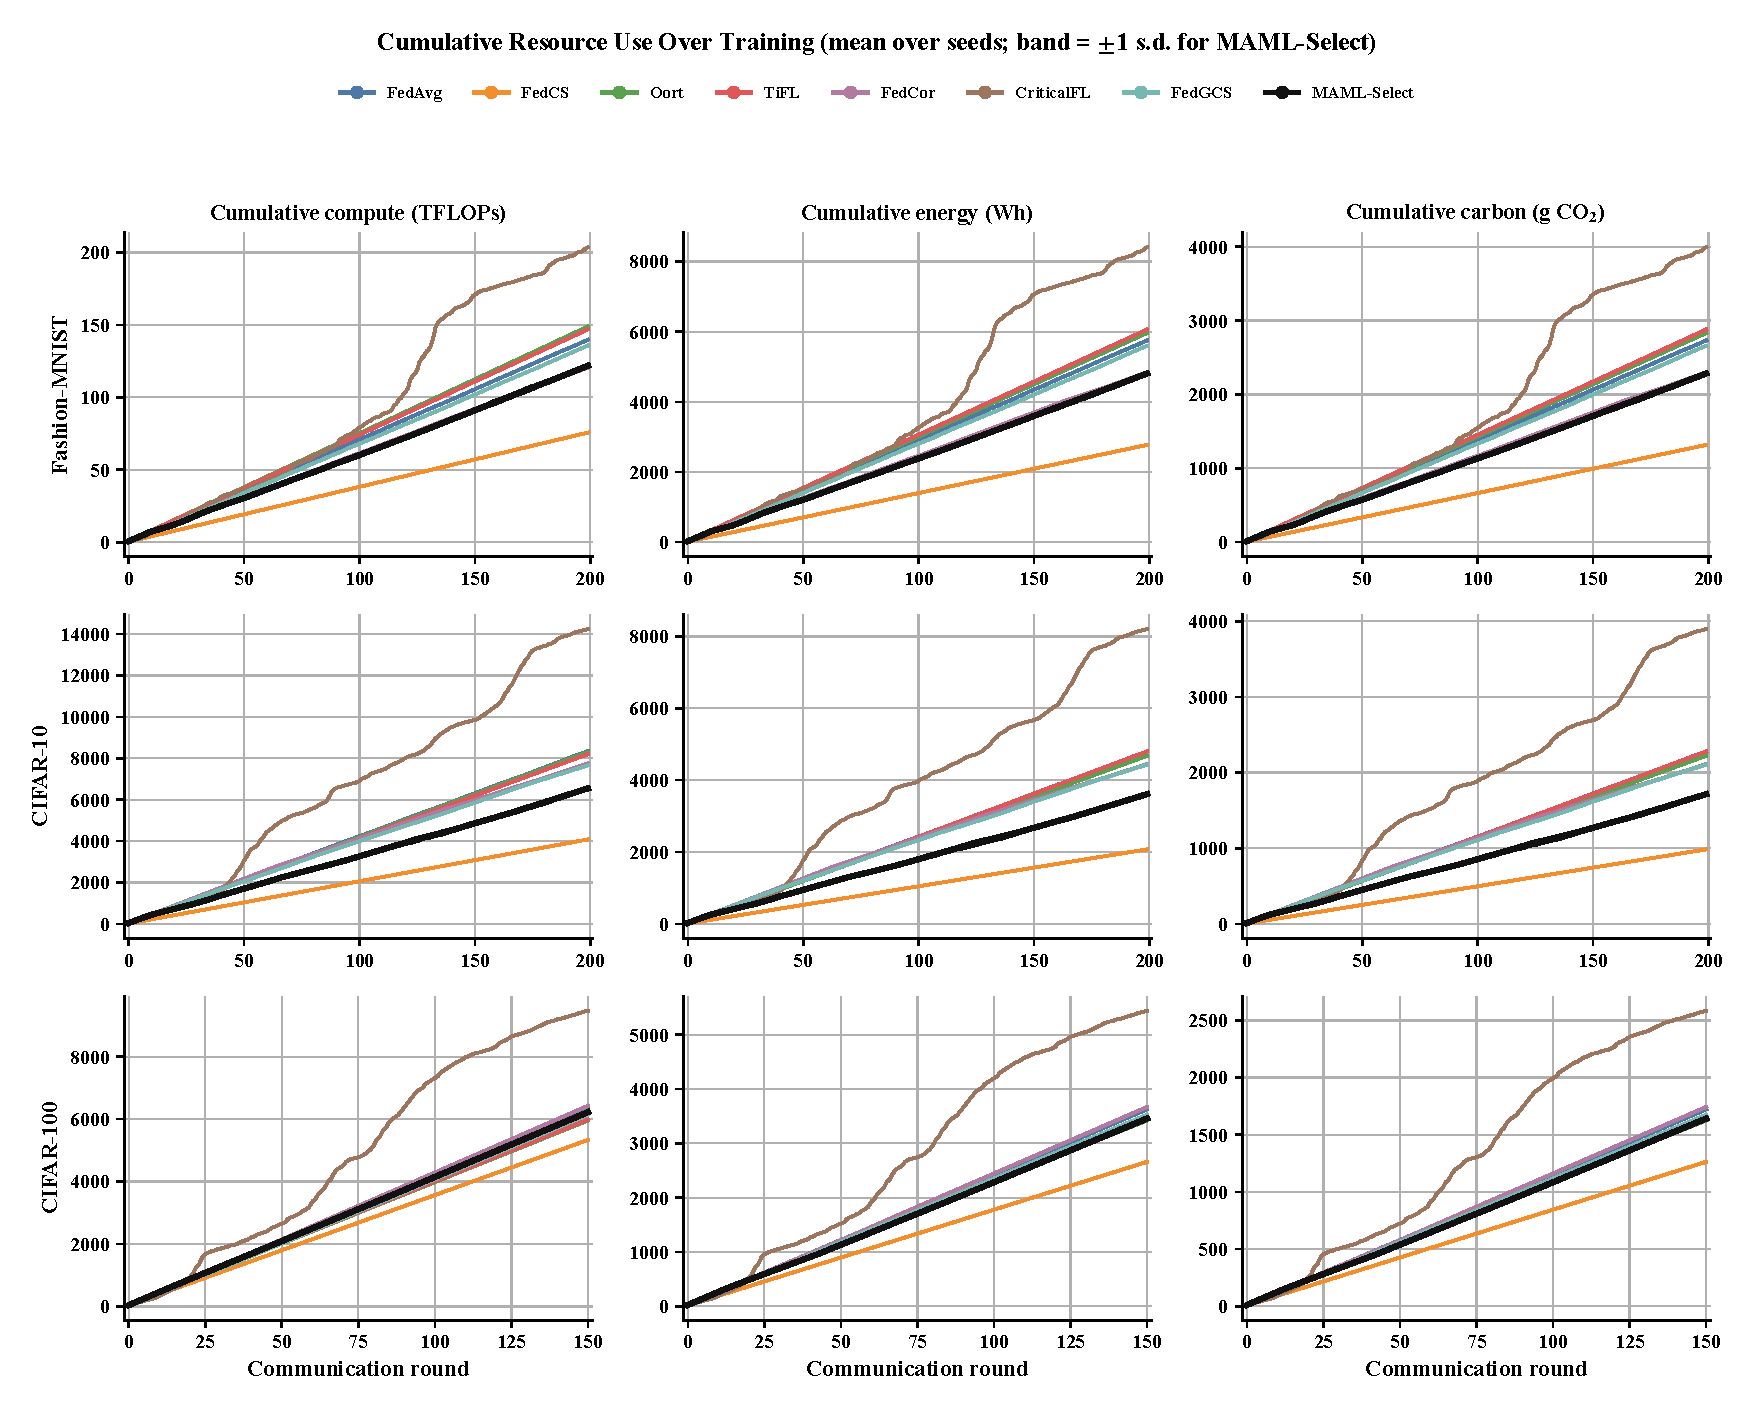
\includegraphics[width=0.92\textwidth]{supp_resource_trajectories}
% \caption{Round-wise cumulative compute and energy trajectories.  The MAML-Select curve remains resource-efficient throughout training, showing that the reported savings are accumulated over the whole FL process rather than appearing only at the final round.}
% \label{fig:supp_resource}
% \end{figure}

\noindent\textbf{Tier-level participation.}\quad
Table~\ref{tab:supp_tier} reports, for each method, the fraction of selections that fall in each device tier, together with client coverage.  The device pool is $20\%$ Tier~1 (slow, $1.0\times$), $50\%$ Tier~2 (medium, $2.0\times$), and $30\%$ Tier~3 (fast, $4.0\times$), so a tier-proportional selector reads $0.20/0.50/0.30$.  Two patterns stand out.  The purely system-aware selectors concentrate on the fast tier and abandon the slow tier: FedCS selects \emph{no} Tier~1 client ($0.00$) and sends $80$ to $83\%$ of its selections to Tier~3, at only $10\%$ coverage.  MAML-Select instead shifts selection toward faster tiers to lower latency and energy (Tier~3 rises to $0.44$ to $0.49$), yet it keeps the slow tier represented ($0.09$) and reaches $100\%$ coverage.  This is the tier-level view of the Jain index and coverage results: MAML-Select is cost-aware but never permanently excludes a tier, unlike the deadline- or utility-constrained baselines.

\begin{table}[!ht]
\centering
\caption{Tier-level selection rates (fraction of selections per device tier) and client coverage, mean over seeds.  Tier~1 slow / Tier~2 medium / Tier~3 fast; pool proportions $0.20/0.50/0.30$.}
\label{tab:supp_tier}
\small
\setlength{\tabcolsep}{6pt}
\begin{tabular}{lcccc}
\toprule
Method & Tier~1 & Tier~2 & Tier~3 & Cov.\ (\%) \\
\midrule
\multicolumn{5}{@{}l}{\textit{Fashion-MNIST}} \\
FedAvg & 0.20 & 0.50 & 0.31 & 100 \\
FedCS & 0.00 & 0.20 & 0.80 & 10 \\
Oort & 0.20 & 0.37 & 0.43 & 10 \\
TiFL & 0.33 & 0.33 & 0.33 & 12 \\
FedCor & 0.16 & 0.44 & 0.41 & 49 \\
CriticalFL & 0.20 & 0.47 & 0.33 & 33 \\
FedGCS & 0.20 & 0.50 & 0.30 & 100 \\
\textbf{MAML-Select} & 0.09 & 0.47 & 0.44 & 100 \\
\addlinespace[2pt]
\multicolumn{5}{@{}l}{\textit{CIFAR-10}} \\
FedAvg & 0.20 & 0.50 & 0.31 & 100 \\
FedCS & 0.00 & 0.17 & 0.83 & 10 \\
Oort & 0.20 & 0.37 & 0.43 & 10 \\
TiFL & 0.33 & 0.33 & 0.33 & 12 \\
FedCor & 0.18 & 0.56 & 0.25 & 31 \\
CriticalFL & 0.20 & 0.48 & 0.32 & 46 \\
FedGCS & 0.22 & 0.47 & 0.31 & 100 \\
\textbf{MAML-Select} & 0.09 & 0.41 & 0.49 & 100 \\
\bottomrule
\end{tabular}
\end{table}

\section*{S3. Sensitivity and State-Feature Ablation}

The sensitivity study evaluates the cost trade-off weight $\lambda\in\{0.1,0.5,1.0,5.0\}$ on Fashion-MNIST.  The selected value $\lambda=0.5$ gives a balanced operating point: accuracy remains close to the best observed value while compute and energy are reduced relative to the low-penalty setting.  The ablation study verifies that the six-dimensional state vector gives stable behaviour; removing one feature at a time changes accuracy only modestly, which indicates that the learned selector is not dependent on a single fragile signal.

\begin{figure}[!ht]
\centering
\begin{minipage}{0.49\textwidth}
\centering
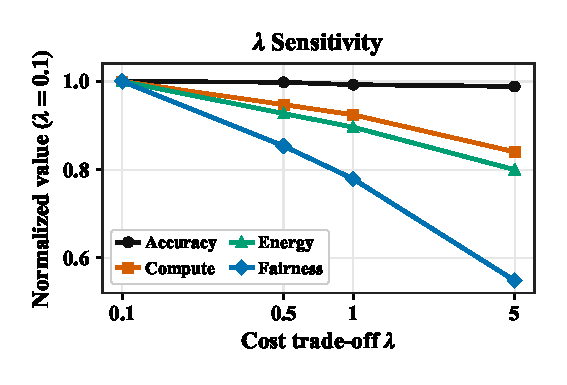
\includegraphics[width=\linewidth]{fig_lambda_sensitivity_multimetric_boxed}
\caption*{(a) $\lambda$ sensitivity.}
\end{minipage}
\hfill
\begin{minipage}{0.49\textwidth}
\centering
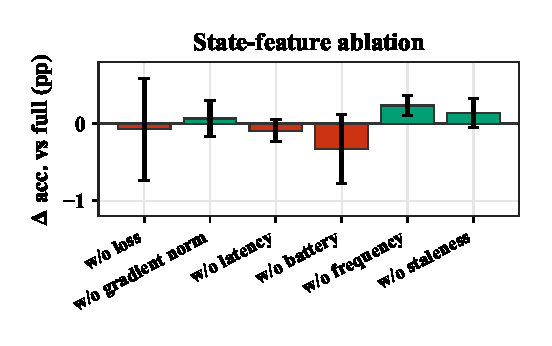
\includegraphics[width=\linewidth]{fig_feature_ablation_trimmed_boxed}
\caption*{(b) State-feature ablation.}
\end{minipage}
\caption{Design evidence for MAML-Select.  The $\lambda$ sweep shows the accuracy--resource trade-off, and the ablation plot shows that the policy remains stable under single-feature removals.}
\label{fig:supp_lambda_ablation}
\end{figure}

\begin{table}[!ht]
\centering
\caption{Fashion-MNIST sensitivity and ablation summaries.}
\label{tab:supp_design}
\footnotesize
\begin{minipage}{0.48\textwidth}
\centering
\begin{tabular}{@{}lrrr@{}}
\toprule
$\lambda$ & Acc. (\%) & TFLOPs & Energy (Wh) \\
\midrule
0.1 & $90.40 \pm 0.22$ & 128.3 & 5176 \\
0.5 & $90.23 \pm 0.55$ & 121.6 & 4799 \\
1.0 & $89.74 \pm 0.79$ & 118.6 & 4639 \\
5.0 & $89.37 \pm 1.02$ & 107.8 & 4140 \\
\bottomrule
\end{tabular}
\end{minipage}
\hfill
\begin{minipage}{0.48\textwidth}
\centering
\begin{tabular}{@{}lrr@{}}
\toprule
Variant & Acc. (\%) & TFLOPs \\
\midrule
Full state & $90.23 \pm 0.55$ & 121.6 \\
w/o loss & $90.16 \pm 0.66$ & 122.8 \\
w/o grad. norm & $90.30 \pm 0.24$ & 122.4 \\
w/o latency & $90.14 \pm 0.14$ & 118.9 \\
w/o battery & $89.90 \pm 0.44$ & 122.2 \\
w/o frequency & $90.47 \pm 0.13$ & 115.0 \\
w/o staleness & $90.37 \pm 0.19$ & 122.7 \\
\bottomrule
\end{tabular}
\end{minipage}
\end{table}

The revised paper adds two further ablations on the selector itself.  The inner-step ablation varies the number of inner adaptation steps on CIFAR-10.  A single step gives the highest accuracy and the lowest selection overhead, which justifies the one-step inner loop.  The selector-width ablation varies the hidden width $h\in\{16,32,64,128\}$ of the $6$-$h$-$h$-$1$ policy on Fashion-MNIST.  Accuracy stays within about $0.6$ points across this $44\times$ parameter range, so the compact $h=64$ default is robust.

\begin{figure}[!ht]
\centering
\begin{minipage}{0.49\textwidth}
\centering
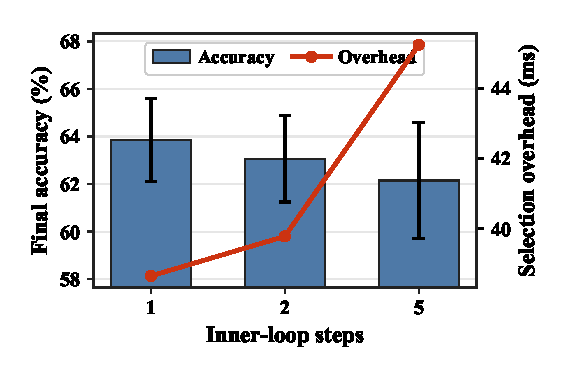
\includegraphics[width=\linewidth]{fig_inner_step_boxed}
\caption*{(a) Inner-loop steps (CIFAR-10).}
\end{minipage}
\hfill
\begin{minipage}{0.49\textwidth}
\centering
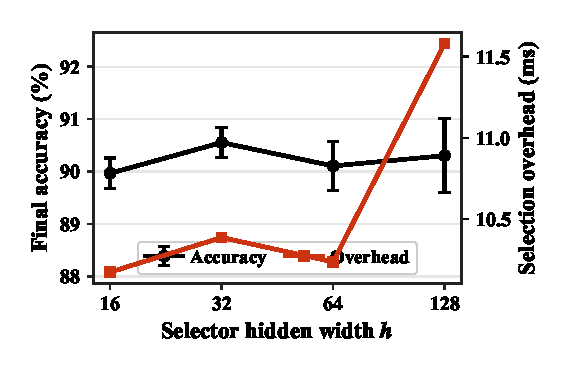
\includegraphics[width=\linewidth]{fig_arch_width_boxed}
\caption*{(b) Selector width (Fashion-MNIST).}
\end{minipage}
\caption{Selector design ablations.  (a) One inner step is the most accurate and lowest-overhead setting.  (b) Accuracy is flat across selector width while overhead grows, so the compact $h=64$ default is sufficient.}
\label{fig:supp_selector_design}
\end{figure}

\section*{S4. Selector Scaling}

The selector-scaling probe runs MAML-Select for $10$ rounds while increasing $N=\{20,40,80,100,200,500,1000\}$ and keeping $K/N=0.1$.  The measured per-round selection overhead stays nearly flat, between about $20$ and $26$~ms, even as $N$ grows fifty-fold to $1000$, and is small compared with local training time.  This supports the complexity argument in the main paper: scoring all available clients with a fixed-size MLP is linear in the client pool, and at these pool sizes that $O(NP)$ cost is dominated by fixed per-round overhead, so the measured time barely changes.

\begin{figure}[!ht]
\centering

\includegraphics[width=0.63\textwidth]{fig_scaling_maml_only_boxed}
\caption{MAML-Select client-selection overhead as the pool size increases, with the selection rate held at $10\%$ ($K/N=0.1$). Panel (b) plots the analytical operation count $C(N,K)=NP+N\log K+2KP$ ($P=4{,}673$), normalized to its value at $N=20$.}
\label{fig:supp_scaling}
\end{figure}

\begin{table}[!ht]
\centering
\caption{Mean MAML-Select selection overhead in seconds, measured over 10 rounds, for client-pool sizes up to $N=1000$ with the selection rate held at $K/N=0.1$.}
\label{tab:supp_scaling}
\small
\setlength{\tabcolsep}{4pt}
\begin{tabular}{@{}lrrrrrrr@{}}
\toprule
Method & $N=20$ & $N=40$ & $N=80$ & $N=100$ & $N=200$ & $N=500$ & $N=1000$ \\
\midrule
MAML-Select & 0.02190 & 0.02189 & 0.01957 & 0.01969 & 0.02493 & 0.02227 & 0.02580 \\
\bottomrule
\end{tabular}
\end{table}

\section*{S5. Extended Algorithm}

Algorithm~\ref{alg:ext} gives the full MAML-Select procedure, expanding Algorithm~1 of the main paper with the state-feature construction, the cold-start rule, the exploration step, and the first-order inner and outer updates. The meta-policy $h_\phi$ is the $6$-$64$-$64$-$1$ MLP. No client raw data leaves the device: the server observes only the six-dimensional state vectors and scalar cost feedback. The procedure is the exact specification used to produce all reported results, so the experiments are reproducible from these steps and the stated hyperparameters.

\begin{algorithm}[!ht]
\caption{MAML-Select (extended)}
\label{alg:ext}
\begin{algorithmic}[1]
\footnotesize
\Require clients $\{1,\dots,N\}$; rounds $T$; cohort $K$; inner LR $\beta$; outer LR $\eta$; trade-off $\lambda$; target latency $T_{\mathrm{target}}$; exploration size $\epsilon$
\State Initialize global model $\theta_1$, meta-policy $\phi_1$, and the Adam state for $\phi$
\State $\mathcal{P}\gets\emptyset$ \Comment{pending feedback from the previous round}
\For{$t=1,\dots,T$}
  \State $\mathcal{A}_t\gets$ clients available this round
  \For{$i\in\mathcal{A}_t$} \Comment{state features}
     \State $\bm{s}_{i,t}\gets[\,\hat{L}_i,\ \lVert\nabla F_i\rVert,\ \hat{T}_i,\ b_i,\ q_i,\ \tau_i\,]$ \Comment{loss, grad-norm, latency, battery, frequency, staleness}
  \EndFor
  \If{$\mathcal{P}\neq\emptyset$} \Comment{inner adaptation and first-order outer update}
     \State $\mathcal{D}_{sup}\gets\{(\bm{s}_{j,t-1},c_{j,t-1}):j\in\mathcal{P}\}$
     \State $\phi'_t\gets\phi_t-\beta\,\nabla_\phi\mathcal{L}(h_\phi;\mathcal{D}_{sup})$ \Comment{one inner step}
     \State $\phi_{t+1}\gets\phi_t-\eta\,\nabla_{\phi'_t}\mathcal{L}(h_{\phi'_t};\mathcal{D}_{sup})$ \Comment{first-order meta-update}
  \Else
     \State $\phi'_t\gets\phi_t$;\quad $\phi_{t+1}\gets\phi_t$
  \EndIf
  \State $\widehat{c}_i\gets h_{\phi'_t}(\bm{s}_{i,t})$ for all $i\in\mathcal{A}_t$ \Comment{score candidates}
  \If{$t\le\lceil N/K\rceil$}
     \State $\mathcal{S}_t\gets$ next $K$ clients in a fixed coverage order \Comment{cold start}
  \Else
     \State $\mathcal{S}_t\gets\mathrm{Top\text{-}}K\ \mathrm{of}\ (-\widehat{c})$, with $\epsilon$ random exploratory clients
  \EndIf
  \State Train selected clients; aggregate $\theta_{t+1}\gets\sum_{i\in\mathcal{S}_t}\tfrac{n_i}{\sum_{j\in\mathcal{S}_t}n_j}\theta_i$ \Comment{FedAvg}
  \For{$i\in\mathcal{S}_t$} \Comment{record cost feedback}
     \State $\rho_i\gets\max(0,T_i-T_{\mathrm{target}})/T_{\mathrm{target}}$ \Comment{normalized latency penalty; $T_i$ is realized latency}
     \State $c_{i,t}\gets\lambda\,\rho_i-\Delta_i$ \Comment{$\Delta_i$: local loss reduction, as in Eq.~(4)}
  \EndFor
  \State $\mathcal{P}\gets\mathcal{S}_t$
\EndFor
\State \Return $\theta_{T+1}$
\end{algorithmic}
\end{algorithm}

\section*{S6. Selector Convergence}

Lemmas~1 and~2 of the main paper give the inner and outer updates a one-step descent property.  Here we draw the standard consequence for the meta-iterates and then verify both properties empirically over training.

\noindent\textbf{Corollary (approximate stationarity).}\quad
Suppose the query objective is shared across rounds, $q_t\equiv q$ with $q$ bounded below by $q^\star$, and Lemma~2 holds with step size $0<\eta\le 1/L_q$.  Summing the per-round descent over $t=1,\dots,T$ and telescoping gives
\[
\min_{1\le t\le T}\lVert\nabla q(\phi_t)\rVert_2^2 \;\le\; \frac{2\,\bigl(q(\phi_1)-q^\star\bigr)}{\eta\,T} \;+\; \frac{1}{T}\sum_{t=1}^{T}\delta_t^2 .
\]
The meta-policy therefore reaches an $\mathcal{O}(\beta^2)$-approximate stationary point at rate $\mathcal{O}(1/(\eta T))$, where the floor is the first-order error $\delta_t^2\le L_q^2\beta^2\lVert\nabla g_t(\phi_t)\rVert_2^2$.  In MAML-Select the query objective is mildly non-stationary because client utility drifts, so the bound describes the slowly-varying regime; we report the empirical behaviour in the general case next.

Fig.~\ref{fig:supp_convergence} verifies the two descent properties during a full training run on each dataset.  Panel~(a) plots the inner-step change $g_t(\phi'_t)-g_t(\phi_t)$; it stays at or below zero in every round ($100\%$ of adapted rounds on all three datasets), confirming Lemma~1.  Panel~(b) plots the query objective relative to its first-round value; it decreases and then stabilizes, which is the empirical signature of outer-loop convergence under the non-stationary target.  Panel~(c) plots the meta-update magnitude $\lVert\phi_{t+1}-\phi_t\rVert_2$; it shrinks and settles, showing that the policy stops moving as it tracks the utility signal.  Together with the global accuracy and loss curves of the main paper, these confirm that the adaptive selector and the federated model both converge in practice, even though a closed-form global guarantee under fully adaptive partial participation remains open.

\begin{figure}[!ht]
\centering
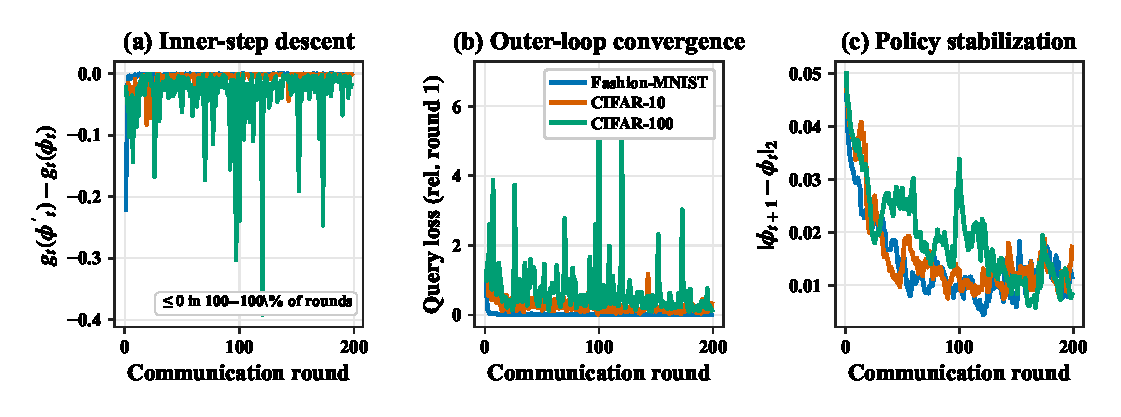
\includegraphics[width=0.98\textwidth]{fig_convergence_verification_boxed}
\caption{Selector-convergence verification over a full training run.  (a)~Inner-step support descent $g_t(\phi'_t)-g_t(\phi_t)\le 0$ (Lemma~1).  (b)~Query objective relative to round~1, decreasing and stabilizing (outer-loop convergence, Lemma~2).  (c)~Meta-update magnitude $\lVert\phi_{t+1}-\phi_t\rVert_2$ shrinking as the policy stabilizes.}
\label{fig:supp_convergence}
\end{figure}

\section*{S7. Summary}

The supplementary evidence strengthens the revised manuscript in five ways.  First, the experimental settings and resource model are fully specified.  Second, MAML-Select shows consistent reductions in modeled compute and energy while retaining full client coverage.  Third, the resource reductions are supported by paired statistical tests over the shared seeds.  Fourth, the sensitivity, ablation, and scaling studies show that the learned selector is tunable, stable under state-feature perturbations, and inexpensive to execute.  Fifth, the tier-level participation analysis shows that MAML-Select keeps every device tier represented while remaining cost-aware, and the convergence study confirms that the inner and outer updates satisfy the proven descent properties and that the selector and global model both converge during training.

\end{document}
